%%%%%%%%%%%%%%%%%%%%%%%%%%%%%%%%%
%% Ersetzen Sie in den folgenden Zeilen die entsprechenden -Texte-
%% mit den richtigen Werten.
\documentclass[course=erap]{aspdoc}
\newcommand{\theGroup}{155} % Beispiel: 42
\newcommand{\theNumber}{A501} % Beispiel: A123
\author{Mete Polat \and Jonas Hübotter \and Simon Martin Bohnen}
\date{Sommersemester 2019} % Beispiel: Wintersemester 2018/19
%%%%%%%%%%%

\usepackage{amssymb}
\usepackage{icomma}
\usepackage{hyperref}
\usepackage{tabularx}
\usepackage[block=ragged]{biblatex}
\addbibresource{bib/Literatur.bib}

% Diese Zeile bitte -nicht- aendern.
\title{Gruppe \theGroup{} -- Abgabe zu Aufgabe \theNumber}

\begin{document}
\maketitle

\section{Einleitung}


\section{Problemstellung und Spezifikation}
\subsection{RC5-16/16/b}

\subsubsection{Schlüsselerweiterung mit P und Q}

Für den Schritt der Schlüsselexpansion von RC5 werden die beiden ungeraden Ganzzahlen $P$ und $Q$ benötigt. Diese sind jeweils für eine gegebene Blockgröße von RC5 konstant. Im Allgemeinen gilt

\begin{equation}
    P = Odd((e - 2) \cdot 2^w)
\end{equation}
\begin{equation}
    Q = Odd((\phi - 1) \cdot 2^w)
\end{equation}

mit $w$ als der Größe eines Halbblocks in Bits, $e$ als der Eulerschen Zahl und $\phi$ als dem Goldenen Schnitt wobei $Odd(x)$ die jeweils näheste ungerade Zahl bezeichnet.\bigbreak

Für RC5-16/16/b --- RC5 mit der Wortgröße $16$, der Rundenanzahl $16$ und der Schlüsselgröße $b$ --- gilt damit:

\begin{align*}
    P &= Odd((2,71828 - 2) \cdot 2^{16}) \\
      &= Odd(0,71828 \cdot 65.536) \\
      &= Odd(47.073,19808) \\
      &= 47.073 \\
      &= 0xb7e1 \\
    Q &= Odd((1,61803 - 1) \cdot 2^{16}) \\
      &= Odd(0,61803 \cdot 65.536) \\
      &= Odd(40.503,21408) \\
      &= 40.503 \\
      &= 0x9e37
\end{align*}

\subsubsection{Sicherheit}
\label{sec:Sicherheit}

Durch die Parametrisierung von RC5\cite[p.2]{rc5rev} unterstützt die Chiffre sowohl unterschiedliche Blockgrößen, unterschiedliche Schlüssellängen als auch eine variable Anzahl von Runden. Hinter dieser Parametrisierung stehen zwei Intentionen:

\begin{enumerate}
    \item Durch die variable Blockgröße soll die Performance von RC5 von neueren 64-Bit Architekturen profitieren --- allerdings nicht auf diese beschränkt sein.\cite[p.1]{rc5rev}
    \item Andererseits sollen die frei wählbaren Parameter $r$ und $b$ dem Nutzer der Chiffre die Entscheidung überlassen, wie viel Sicherheit und welche Performance seine Applikation benötigt.\cite[p.1]{rc5rev}
\end{enumerate}

Damit sind zur Beurteilung der Sicherheit von RC5 im Allgemeinen insbesondere die Rundenanzahl und die Schlüssellänge zu betrachten. Die Sicherheit von RC5-16/16/b ist auch von der Blockgröße abhängig.

\paragraph{Schlüssellänge} So wie im Allgemeinen bei Blockchiffren ist auch bei RC5 die Sicherheit der Chiffre stark von der gewählten Schlüssellänge abhängig. RC5 hat den Parameter $b$ mit $b \in \{k \in \mathbb{N}_0 \colon k \leq 255\}$, der die Länge des Schlüssels in Bytes angibt.\cite[p.3]{rc5rev} Die Länge der erweiterten Schlüsseltabelle in Bits ergibt sich durch $2^{(2r + 2)w}$.\cite[p.2]{rc5rev} Der Aufwand für eine \textit{erschöpfende Suche} ist damit $min\{2^{8b}, 2^{(2r + 2)w}\}$.\cite[p.29]{kaliski+yin} Für RC5-16/16/b ist damit der Aufwand einer erschöpfenden Suche allein von $b$ abhängig, solange $b < 68$ gilt.\bigbreak

Das Bundesamt für Sicherheit in der Informationstechnik (BSI) schlägt für Blockchiffren wie RC5 eine minimale Schlüssellänge von $128$ Bits vor.\cite[p.21]{bsi}

\paragraph{Betriebsmodus} In der Praxis werden Blockchiffren in der Regel mit einem Betriebsmodus umgesetzt, mithilfe dessen auch Nachrichten variabler Länge verschlüsselt werden können. Entscheidend ist für deren Sicherheit, dass der entstehende Ciphertext pseudorandom ist.\bigbreak

Ist dies nicht der Fall --- resultieren äquivalente Plaintext-Blöcke beispielsweise in äquivalenten Ciphertext-Blöcken ---, dann enthält der Ciphertext Informationen zur Struktur des Plaintextes\cite[p.22]{bsi}. In diesem Fall können Teile des Plaintextes durch \textit{Häufigkeitsanalyse} rekonstruiert werden\cite[p.22]{bsi}, oder sogar der verwendete Schlüssel durch einen \textit{Codebook Attack} gewonnen werden\cite[p.2]{elbaz}.\bigbreak

Sichere Operationsmodi sind beispielsweise \textit{Counter Block Chaining (CBC)} und der \textit{Counter Mode (CTR)}, da dort der $n$-te Chiphertext-Block nicht nur von dem $n$-ten Plaintext-Block und dem genutzten Schlüssel abhängt, sondern zudem noch von einem weiteren Wert, wie dem $(n-1)$-ten Ciphertext-Block oder einem Zähler.\cite[p.22]{bsi}

\paragraph{Rundenanzahl} Nach Kaliski und Yin werden für eine \textit{differenzielle Kryptoanalyse} von RC5-32/16/b entweder $2^{61}$ selbst gewählte Plaintexte oder $2^{63}$ bekannte Plaintexte benötigt. Ein solcher Angriff auf ein $16$-rundiges RC5 ist damit überaus unwahrscheinlich. Da die Anzahl der möglichen Plaintexte bei dieser Konfiguration von RC5 jedoch bei $2^{64}$ liegt, kann ein solcher Angriff nicht theoretisch ausgeschlossen werden.\cite[p.6]{kaliski+yin} Weiterhin sei eine \textit{lineare Kryptoanalyse von RC5} nur bei einer sehr geringen Rundenzahl von RC5 effektiv.\cite[p.28]{kaliski+yin}\bigbreak

Knudsen und Meier zeigen zwar, dass die Komplexität des von Kaliski und Yin vorgeschlagenen differenziellen Angriffs um einen Faktor von bis zu $512$ reduziert werden kann.\cite[p.2]{knudsen+meier} Allerdings bleibt ein solcher Angriff damit weiterhin sehr unwahrscheinlich. Zudem wurde gezeigt, dass für bestimmte Teile des Schlüsselraums die differentiellen Kryptoanalysen weiter verbessert werden können.\cite[p.13]{knudsen+meier} Allerdings sind für einen effektiven Angriff entweder zu wenige Schlüssel betroffen oder die Anzahl der benötigten Plaintexte weiterhin zu hoch. Heys konnte Ähnliches für lineare Kryptoanalyse zeigen.\cite[p.5]{heys}\bigbreak

\paragraph{Blockgröße} Durch die $32$ Bit Blockgröße von RC5-16/16/b ist die Komplexität eines \textit{generischen Angriffs} durch $2^{32}$ nach oben beschränkt. Damit kann eine untere Schranke $\epsilon$ für die Wahrscheinlichkeit eines Angriffs abgeschätzt werden durch

\[
    \epsilon \geq \frac{\sigma^2}{2^n}
\]

wobei $\sigma$ der Anahl der verarbeiteten Blöcke und $n = 2w$ der Blockgröße entspricht.\bigbreak

Die minimale Wahrscheinlichkeit eines generischen Angriffs auf eine 32-Bit Blockchiffre ist somit $2^{-32}$. Aus diesem Grund eignen sich $32$-Bit Blockchiffren im Allgemeinen und RC5-16/16/b im Speziellen nicht für die Verschlüsselung von großen Datenmengen.\bigbreak

Die RC5 Chiffre kann damit bei für die Anwendung ausreichend großer Blockgröße und Rundenanzahl, $b >= 16$ und Nutzung eines geeigneten Betriebsmodus als sicher gelten. RC5-16/16/b eignet sich lediglich zur Verschlüsselung von kleinen Datenmengen.

\subsection{Feistelchiffren}

Die folgende allgemeine Darstellung von Feistelchiffren soll auf klassische (auch ausgewogene) Feistelchiffren begrenzt werden. Wie für RC5, gilt für klassische Feistelchiffren, dass die Längen der beiden Halbblöcke eines Blocks gleich sein müssen. Zudem wird sich auf das für die umkehrbare Verknüpfung von zwei Halbblöcken übliche $\oplus$ (XOR) beschränkt.

\subsubsection{Einrundige Feistelnetzwerke}

Eine Feistelchiffre ist eine rundenbasierte Blockchiffre, die nach der Art eines Feistelnetzwerks aufgebaut ist. Sei
\[
    F_n := \{f \mid f \colon \{0, 1\}^n \to \{0, 1\}^n\}
\]
die Famile der Rundenfunktionen. Zunächst soll ein klassisches einrundiges Feistelnetzwerk $\Psi$ betrachtet werden. Dieses wird definiert durch eine beliebige Abbildung $f \in F_n$ und eine umkehrbare Bitoperation --- durch obige Einschränkung der Allgemeinheit $\oplus$.
\[
    \Psi(f) \colon \{0, 1\}^{2n} \to \{0, 1\}^{2n} \colon [L, R] \mapsto [S, T] \Leftrightarrow
        \begin{cases}
            S = R \\
            T = L \oplus f(R) \\
        \end{cases}
\]
für $\forall(L, R) \in (\{0, 1\}^n)^2$.\cite[p.11]{nachef}

\begin{center}
    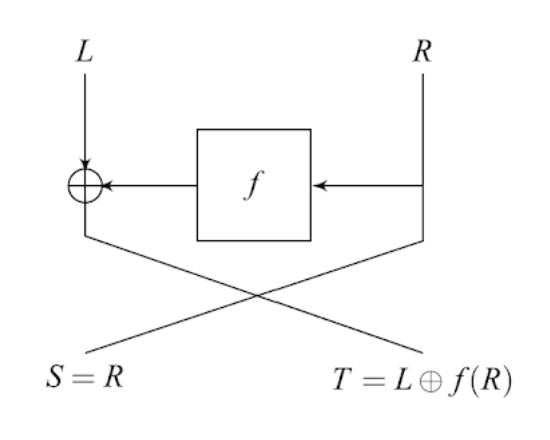
\includegraphics[scale=1]{img/1_round_feistel_cipher_enc.png}\break
    \cite[Fig. 2.1]{nachef}
\end{center}

Wichtig für jede Verschlüsselung ist Bijektivität, damit jedem Codewort eine eindeutige Plaintext-Nachricht zugeordnet werden kann. $\Psi(f)$ ist unabhängig von $f \in F_n$ eine Permutation, d.h. $f$ selbst muss nicht bijektiv sein.\cite[p.12]{nachef}\bigbreak

Aus der Definition von $\Psi(f)$ ergibt sich ihr Inverses als
\[
    \Psi(f)^{-1} = \sigma \circ \Psi(f) \circ \sigma
\]
mit $\sigma$ definiert als $\sigma([L, R]) = [R, L]$ für $L, R \in \{0, 1\}^n$, der Vertauschung beider Halbblöcke.\cite[p.12]{nachef}

\begin{center}
    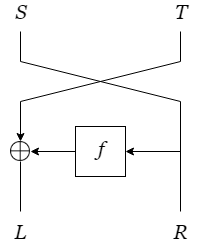
\includegraphics[scale=0.5]{img/1_round_feistel_cipher_dec.png}
\end{center}

\subsubsection{r-rundige Feistelnetzwerke}

Üblicherweise werden Feistelnetzwerke in mehreren Runden angewendet. Im Allgemeinen ist ein klassisches Feistelnetzwerk mit $r \geq 1$ Runden und $f_1, f_2, ..., f_r \in F_n$ Rundenfunktionen definiert durch
\[
    \Psi^r(f_1, ..., f_r) = \Psi(f_r) \circ ... \circ \Psi(f_2) \circ \Psi(f_1).
\]\cite[p.12]{nachef}

\begin{center}
    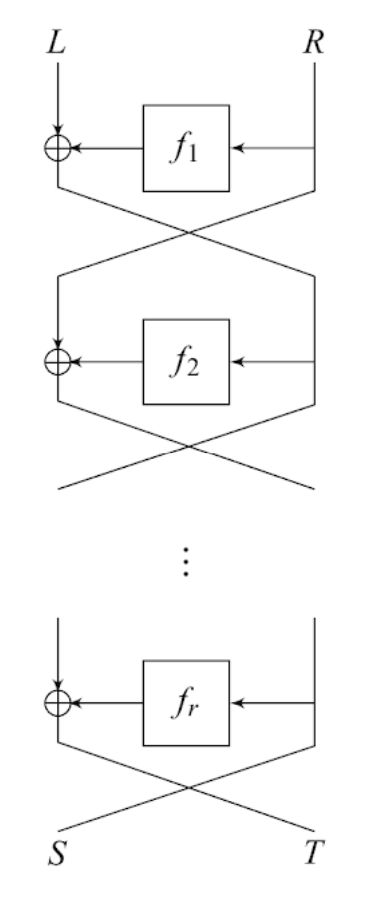
\includegraphics[scale=1]{img/r_round_feistel_cipher_enc.png}\break
    \cite[Fig. 2.2]{nachef}
\end{center}

Da ein einrundiges Feistelnetzwerk eine Permutation über $\{0,1\}^{2n}$ ist, sind auch $r$-rundige Feistelnetzwerke Permutationen. Weiterhin ist das Inverse eines $r$-rundigen Feistelnetzwerks die Komposition der Inversen der einzelnen Runden.
\begin{align*}
    (\Psi^r(f_1, ..., f_r))^{-1} &= \sigma \circ \Psi(f_1) \circ \sigma \circ ... \circ \sigma \circ \Psi(f_r) \circ \sigma \\
                                 &= \sigma \circ \Psi^r(f_r, ..., f_1) \circ \sigma
\end{align*}\cite[p.13]{nachef}\bigbreak

Eine Feistelchiffre ist nun ein spezielles Feistelnetzwerk, dessen Rundenfunktionen von einem Rundenschlüssel aus dem Schlüsselraum $K$ abhängen.
Seien die Rundenschlüssel $(k_1, ..., k_r) \in K^r$ und die Familie der Rundenfunktionen
\[
    F_{n, K} := \{f_k \mid k \in K, f_k \colon \{0, 1\}^n \to \{0, 1\}^n\}.
\]
Dann ist eine Feistelchiffre das Feistelnetzwerk $\Psi^r(f_{k_1},...,f_{k_r})$. Also die $r$-rundige Permutation von der Nachricht $\{0, 1\}^{2n}$ in Abhängigkeit vom Schlüssel $(k_1, ..., k_r)$.\cite[p.14]{nachef}

\subsubsection{RC5 als Feistelchiffre}

RC5 ist eine symmetrische Blockchiffre, deren Aufbau dem einer Feistelchiffre gleicht. RC5 hat die Parameter:\cite[p.2f]{rc5rev}

\begin{itemize}
    \item $w$ ist die Wortgröße in Bits. Ein durch RC5 verschlüsselbarer Block besteht aus zwei Wörtern.
    \item $r$ ist die Anzahl der Runden in denen RC5 Operationen auf einem Block ausführt. Jede Runde besteht aus zwei Halbrunden, in denen ein Wort aus dem Block alteriert wird.
    \item $b$ ist die Anzahl der Bytes in dem privaten Schlüssel $K$.
\end{itemize}

RC5 baut zu Beginn die erweiterte Schlüsseltabelle $S$ auf, die aus $2r + 2$ Schlüsseln besteht und von $K$ abhängt. Seien $\Sigma := (S_2, S_3, ..., S_{2r+1}) = (\Sigma_0, \Sigma_1, ..., \Sigma_{2r-1})$ mit $|\Sigma| = 2r$ die Schlüssel aus der erweiterten Schlüsseltabelle, die während der Runden von RC5 zum Verschlüsseln benutzt werden --- $S_0$ und $S_1$ werden für das Key-Whitening genutzt. Zudem sei $(g_{\Sigma_0}, g_{\Sigma_1}, ..., g_{\Sigma_{2r-1}})$ definiert durch
\begin{align*}
    g_k \colon &\{0, 1\}^w \times \{0, 1\}^w \to \{0, 1\}^w \colon \\
               &(\tau, R) \mapsto (\tau \lll R) + k
\end{align*}
mit $\tau = L \oplus R$, $k \in \Sigma$ und $L, R \in \{0, 1\}^w$ wobei $x \lll y$ die Linksrotation von $x$ um $y$ Bits angibt. Dann zeigt die folgende Tabelle die Zusammenhänge von RC5 und Feistelchiffren.

\begin{center}
 \begin{tabular}{c|c}
 RC5 & Feistelchiffre \\
 \hline
 $r$ & $2r$ \\
 $w$ & $n$ \\
 $\Sigma$ & $K^{2r}$ \\
 $(g_{\Sigma_0}, g_{\Sigma_1}, ..., g_{\Sigma_{2r-1}})$ & $(f_{k_1}, ..., f_{k_{2r}}) \in F^{2r}_{n, K}$ \\
\end{tabular}
\end{center}

Die Reihenfolge der Anwendung der umkehrbaren Bitoperation ($\oplus$) und der Rundenfunktion unterscheidet sich leicht zwischen RC5 und einer allgemeinen klassischen Feistelchiffre. Dieser Unterschied soll in der folgenden Abbildung skizziert werden.

\begin{samepage}
\begin{center}
    \includegraphics[scale=0.5]{img/rc5_feistel_cipher.png}\break
    \textit{Links eine Runde einer Feistelchiffre, rechts eine Runde (zwei Halbrunden) von RC5.}
\end{center}
\end{samepage}

wobei $r$ die aktuelle Runde angibt. Wie dargestellt, ist eine Halbrunde von RC5 im Aufbau ähnlich zu einer Runde einer Feistelchiffre.\bigbreak

Durch den leicht modifizierten Aufbau einer Feistelchiffre in RC5, verändert sich bei RC5 die Berechnung der Inversen. Für eine RC5-Runde gilt
\[
    RC5_{r, \Sigma} \colon \{0, 1\}^{2w} \to \{0, 1\}^{2w} \colon [L, R] \mapsto [S, T] \Leftrightarrow
        \begin{cases}
            S = ((L \oplus R) \lll R) + \Sigma_{2r-2} \\
            T = ((R \oplus S) \lll S) + \Sigma_{2r-1} \\
        \end{cases}.
\]
Damit gilt für die Berechnung der Inversen von einer RC5-Runde
\[
    RC5_{r, \Sigma}^{-1} \colon \{0, 1\}^{2w} \to \{0, 1\}^{2w} \colon [S, T] \mapsto [L, R] \Leftrightarrow
        \begin{cases}
            L = ((S - \Sigma_{2r-2}) \ggg R) \oplus R \\
            R = ((T - \Sigma_{2r-1}) \ggg S) \oplus S \\
        \end{cases}
\]
für $\forall(S, T) \in (\{0, 1\}^w)^2$ wobei $x \ggg y$ die Rechtsrotation von $x$ um $y$ Bits angibt.

\subsection{PKCS\#7-Padding}

Da eine Blockchiffre nur Nachrichten vollständig verschlüsseln kann, die restfrei in Blöcke geteilt werden können, muss die Länge dieser Nachrichten zunächst auf ein Vielfaches der Blockgröße erweitert werden. Diese Erweiterung wird im Allgemeinen als Padding bezeichnet.\bigbreak

Das PKCS\#7-Padding ist eine Form der Erweiterung des Plaintextes auf ein Vielfaches der Blocklänge und soll im Folgenden erläutert werden. Es sei $\Delta$ definiert als
\[
    \Delta = b - (l \bmod b)
\]
mit $b$ als der Länge eines Blocks und $l$ als der Länge des Plaintextes in Byte. Vor der Anwendung eines Verschlüsselungsalgorithmus, der als Länge des Inputs ein Vielfaches von $b$ Bytes erwartet, werden $\Delta$ Bytes jeweils mit dem Wert $\Delta$ an den Plaintext angefügt.\cite[p.28]{rfc5652}\bigbreak

Das heißt, dass der Input in Abhängigkeit von $b$ und $l$ um eine der folgenden Byte-Sequenzen erweitert wird:

\begin{samepage}
\begin{verbatim}
         01 -- if l mod b = b-1
      02 02 -- if l mod b = b-2
          .
          .
          .
b b ... b b -- if l mod b = 0
\end{verbatim}
\end{samepage}

Nach dem Entschlüsseln des Codewortes, kann das Padding auf eindeutige Weise entfernt werden, da jeder Plaintext --- einschließlich jener, deren Länge selbst ein Vielfaches der Blockgröße ist --- vor der Verschlüsselung mit PKCS\#7-Padding erweitert wurde. Die Anzahl der zu entfernenden Bytes wird durch das letzte Byte des letzten Blocks angegeben. PKCS\#7-Padding ist wohldefiniert für $b < 256$.\cite[p.28]{rfc5652}

\section{Lösungsfindung}

\subsection{Initialisierungsvektor}
\label{sec:Initialisierungsvektor}
Eine Herausforderung ist die Erzeugung und Speicherung des Initialisierungsvektors, der beim Cipher Block Chaining Mode benötigt wird. Es ist einerseits entscheidend, dass dieser nicht aus zuvor bekannten Informationen erzeugt wird, wie es zum Beispiel bei SSL 3.0 und TLS 1.0 der Fall war. Dort führte dies zu einer Schwäche, falls dem Angreifer zwei aufeinanderfolgende Ciphertext-Blöcke bekannt waren \cite{ssltls}. Andererseits ist eine ausreichende Länge wichtig, um einem Related-Key-Attack vorzubeugen, der zum Beispiel das WEP-Protokoll betraf \cite{wep}.\bigbreak

Aufgrund der Blocklänge bietet sich nur ein 32-Bit-Initialisierungsvektor an, der pseudozufällig generiert wird.
Eine Geheimhaltung des Initialisierungsvektors ist nicht erforderlich \cite[p.194]{appcrypt}, weshalb der Vektor am Ende der verschlüsselten Datei gespeichert und dort bei der Entschlüsselung wieder ausgelesen wird.

\subsection{Einmaliges Ausführen der Schlüsselexpansion}
Ein bei gleicher Rundenanzahl und Blockgröße stets gleich bleibender Schritt bei der Ver- und Entschlüsselung ist die Schlüsselexpansion. Diese hängt nur von den Nothing-Up-My-Sleeve-Zahlen $P$ und $Q$ ab und muss daher im Voraus nur einmal berechnet werden. Die resultierenden Rundenschlüssel werden in der data-Section unseres Assemblyprogramms gespeichert, um sie beim Key-Mixing weiterzuverwenden. Der Code zur Schlüsselexpansion ist seperat in der Datei key\_expansion.S zu finden.

\subsection{Optimierung durch SIMD}
Eine Optimierung durch SIMD ist möglich und sinnvoll, wenn ein Algorithmus auf mehreren Datenblöcken die selbe Operation ohne Abhängigkeiten zwischen Blöcken ausführt. Bei RC5 und dem CBC-Mode werden jedoch häufig Abhängigkeiten verwendet, um statistischen Analysen, wie sie zum Beispiel beim ECB-Mode möglich sind, vorzubeugen.\bigbreak

Beim Key-Mixing hängt der nächste Rundenschlüssel beispielsweise direkt vom vorherigen ab, wodurch eine Parallelisierung unmöglich wird.
Ähnliches gilt für die Ver- und Entschlüsselung, da dort zur Erzeugung des nächsten Ciphertextblocks der vorherige benötigt wird.\bigbreak

Die einzig mögliche Optimierung ist das gleichzeitige Laden mehrerer Rundenschlüssel oder Blöcke aus dem Speicher, um die Anzahl der Zugriffe zu minimieren. Zunächst war unser Ziel, mit SSE-, AVX- oder AVX-512-Registern möglichst viele Schlüssel gleichzeitig zu laden. Für die Benutzung bei der Ver-/Entschlüsselung werden jedoch einzelne Schlüssel benötigt. Da die x86-64-Instruktion PEXTRW, die das Extrahieren einer einzelnen Lane erlaubt, als Laneindex nur einen Immediate akzeptiert, entschieden wir uns, 4 Schlüssel gleichzeitig in ein 64-Bit-Register zu laden und durch Shift-Operation den passenden Schlüssel in die niedrigen 16 Bit zu bewegen.

\section{Dokumentation der Implementierung}
Die hier bereitgestellte RC5-Implementierung kann zur sicheren Ver- und Entschlüsselung von Daten
genutzt werden.
Voraussetzung dafür, ist das Wählen eines geeigneten Schlüssels mit mindestens 16 Byte Länge (siehe
\hyperref[sec:Sicherheit]{2.1.2 Sicherheit}).
Es stehen die Betriebsmodi Cipher Block Chaining (CBC) und Counter Mode (CTR) zur Verfügung, wobei
letzterer effizienter ist.\bigbreak

Im Folgenden ist die Gebrauchsanweisung der RC5-Implementierung beschrieben:

\begin{verbatim}
    rc5 (-d | --decrypt | -e | --encrypt) [--ctr] <key> <inputFile> [outputFile]
\end{verbatim}
Es kann entweder verschlüsselt oder entschlüsselt werden.
Falls beide Optionen angegeben sind, bricht das Programm ab.
Sofern keine Ausgabedatei angegeben ist, wird das Ergebnis in die Eingabedatei geschrieben.

\subsection{Entwicklerdokumentation}

\subsubsection{Funktionen}

\begin{verbatim}
int main(int argc, char **argv)
\end{verbatim}
Liest übergebene Parameter aus und bestimmt den Programmfluss.\\[1.5mm]
\texttt{argc} Die Anzahl der übergebenen Parameter inklusive Programmaufrufname.\\
\texttt{argv} Die übergebenen Parameter.
Der Programmaufrufname ist an erster Stelle.\\
\begin{verbatim}
void usage(const char *restrict program_name)
\end{verbatim}
Gibt die in der Benutzerdokumentation angegebene Gebrauchsanweisung aus.\\[1.5mm]
\texttt{program\_name} Programmname.
Wird mit ausgegeben.\\
\begin{verbatim}
long read_file(const char *restrict path, void *restrict buffer, size_t size)
\end{verbatim}
Liest die Datei in \texttt{path} in \texttt{buffer}.\\[1.5mm]
\texttt{path} Der Pfad zur Datei, die gelesen werden soll.\\
\texttt{buffer} Der Buffer in dem die Datei gespeichert werden soll.
Wenn \texttt{NULL}, gibt die Funktion die Dateigröße in Bytes zurück.\\
\texttt{size} Die Größe des Buffers.\\
\texttt{return} Gibt die Dateigröße in Bytes zurück wenn buffer \texttt{NULL} ist, ansonsten wird
\texttt{0} zurückgegeben.
Falls ein Fehler auftritt, wird \texttt{-1} zurückgegeben.\\
\begin{verbatim}
int write_file(const char *restrict path, const void *restrict buffer, size_t size)
\end{verbatim}
Speichert \texttt{buffer} an den angegeben Pfad.\\[1.5mm]
\texttt{path} Der Pfad an den buffer gespeichert werden soll.\\
\texttt{buffer} Der Buffer, der die zu speichernden Daten enthält.\\
\texttt{size} Die Größe des Buffers\\
\texttt{return} Gibt \texttt{0} zurück wenn erfolgreich, ansonsten \texttt{-1}.\\
\begin{verbatim}
void cleanup(void)
\end{verbatim}
Wird aufgerufen sobald das Programm terminiert.
Räumt falls nötig einen in der \texttt{main}-Methode allokierten Buffer auf.\\
\begin{verbatim}
void fclose_keep_errno(FILE *file)
\end{verbatim}
Helfermethode, die eine Datei schließt und dabei den Wert von errno beibehält.
Hilfreich falls \texttt{fclose(file)} aufgrund eines vorangegangenen Fehlers aufgerufen werden
soll, aber \texttt{fclose} nicht den Fehlercode überschreiben soll, falls es auch in dieser zu
einem Fehler kommt.\\
Hinweis: Die errno Variable ist in der \texttt{errno.h} definiert.
Sie wird von verschiedenen Funktionen wie \texttt{fopen()} oder \texttt{ftell()} gesetzt, sobald
es zu einem Fehler kommt und kann dann benutzt werden um den genauen Fehlergrund auszulesen.\\
[1.5mm]
\texttt{file} Die durch \texttt{fclose()} zu schließende Datei.\\
\begin{verbatim}
void pkcs7_pad(void *buf, size_t len)
\end{verbatim}
Fügt an \texttt{buf} \texttt{len} Bytes hinzu mit \texttt{len} als Inhalt.\\[1.5mm]
\texttt{buf} Die Stelle an der das Padding hinzugefügt werden soll.\\
\texttt{len} Die Anzahl an Bytes die hinzugefügt werden sollen.\\
\begin{verbatim}
void rc5_cbc_enc(unsigned char *key, size_t keylen, uint32_t *buffer,
                 size_t len, uint32_t iv)
\end{verbatim}
Verschlüsselt die Daten mithilfe des Cipher Block Chaining (CBC) Modes.\\[1.5mm]
\texttt{key} Der Schlüssel zum Verschlüsseln der Datei.\\
\texttt{keylen} Die Schlüssellänge.\\
\texttt{buffer} Die zu verschlüsselnden Daten inklusive dem Padding.\\
\texttt{len} Die Länge des Buffers.\\
\texttt{iv} Ein zufälliger Initialisierungsvektor.\\
\begin{verbatim}
int rc5_cbc_dec(unsigned char *key, size_t keylen, uint32_t *buffer,
                size_t len, uint32_t iv)
\end{verbatim}
Entschlüsselt die Daten mithilfe des Cipher Block Chaining (CBC) Modes.\\[1.5mm]
\texttt{key} Der Schlüssel zum Entschlüsseln der Datei.\\
\texttt{keylen} Die Schlüssellänge.\\
\texttt{buffer} Die zu entschlüsselnden Daten inklusive dem Padding.\\
\texttt{len} Die Länge des Buffers.\\
\texttt{iv} Der Initialisierungsvektor mit dem die Datei verschlüsselt wurde.\\
\texttt{return} Die Anzahl der entschlüsselten Bytes ohne Padding.\\
\begin{verbatim}
void rc5_init(unsigned char *key, size_t keylen, void *l)
\end{verbatim}
Führt das Keysetup durch.\\[1.5mm]
Die ursprüngliche Methodendefinition aus der Angabe wurde hier bearbeitet.
Der Parameter \texttt{void *s} wurde entfernt.
Dieser zeigte auf allokierten Speicherbereich, in welchem die erweiterte Schlüsseltabelle nach
Berechnung abgelegt werden konnte.
Die Schlüsseltabelle ändert sich jedoch aufgrund der festgesetzten Parameter (RC5-16/16/b) nicht
und wird deswegen vorberechnet in der \texttt{.data}-Sektion gespeichert.
Die ursprüngliche Berechnung wurde mit \texttt{key\_expansion.S} und \texttt{objdump}
durchgeführt.\\[1.5mm]
\texttt{key} Der Schlüssel zum ver- oder entschlüsseln der Datei.\\
\texttt{keylen} Die Schlüssellänge.\\
\texttt{l} L ist der Pointer auf das Array aus 16-Bit Worten bestehend aus dem Schlüssel, der
gegebenenfalls mit Nullen aufgefüllt wird.
\begin{verbatim}
void rc5_enc(uint32_t *buffer)
\end{verbatim}
Führt die eigentliche RC5 Verschlüsselung auf einem 32-Bit Block durch.\\[1.5mm]
\texttt{buffer} Adresse auf 4 Bytes, die verschlüsselt werden sollen.\\
\begin{verbatim}
void rc5_dec(uint32_t *buffer)
\end{verbatim}
Führt die eigentliche RC5 Entschlüsselung auf einem 32-Bit Block durch.\\[1.5mm]
\texttt{buffer} Adresse auf 4 Bytes, die entschlüsselt werden sollen.

\subsection{Dateiaufbau}
Im Folgenden ist der Aufbau einer von der RC5-Implementierung verschlüsselten Datei aufgezeigt,
wobei der Initialisierungsvektor selbst nicht verschlüsselt wird.\\[1.5mm]
\begin{tabularx}{\textwidth}{|X|X|X|}
    \hline
    \centering Plaintext & \centering Padding & \centering\arraybackslash Initialisierungsvektor\\
    \hline
\end{tabularx}\\[1.5mm]
Siehe \hyperref[sec:Initialisierungsvektor]{3.1 Initialisierungsvektor} für dessen nähere
Beschreibung.

\section{Ergebnisse}



\subsection{Performance}

\section{Zusammenfassung}

\printbibliography

\end{document}

